\chapter{Introduction}
\label{ch-1}
\begin{refsection}[refs/ch-1.bib]
This thesis examines methods to include environmental impacts in health technology assessment (HTA), and this chapter introduces the key concepts underpinning its content. First, it describes how decisions in the healthcare system are made, introducing HTA and health economic evaluation. Second, it outlines the relationship between healthcare decisions and the environment, introducing the health impacts of climate change and healthcare sustainability. Third, it summarises existing work to include environmental impacts in HTA. It concludes with the objectives of the thesis.

\section{Making decisions in the health system}
Decisions about the health system are made daily. Patients must decide when to seek care, clinicians must decide what care to recommend, and those responsible for the funding and delivery of the health system must decide what care is made available for use. Drummond et al. characterise these as decisions of resource allocation—“who should do what to whom, with what healthcare resources, and with what relation to other health services.”\cite{drummond_methods_2015} This thesis focuses on decisions about which services, tests, and treatments receive Federal Government reimbursement to make them affordable at the point of care.

The remainder of this thesis refers to health services, tests, and treatments as \textit{technologies}, being “an intervention developed to prevent, diagnose or treat medical conditions; promote health; provide rehabilitation; or organise health delivery".\cite{orourke_new_2020} The intervention can be a test, device, medicine, vaccine, procedure, program, or system.\cite{orourke_new_2020}

Government reimbursement decisions about health technologies are made based on the \textit{opportunity cost} of those decisions equal to the value of the forgone use of those same resources. Imagine a world where there is no scarcity and the various resources required to deliver healthcare are unlimited. In this world decisions might only concern whether a technology is safe and expected to have health benefits. There would be no concern of resource depletion, as resources could be spent without consideration of their alternative use. However, this is not the world we live in, and the money, people, time, and energy required to deliver healthcare are finite and scarce. Therefore, when decisions are made to spend resources, they are done so at the expense of all other alternative use of those resources—their opportunity cost.

In many countries, including Australia, government healthcare reimbursement decisions are made based on opportunity costs. The methods used to inform decisions about opportunity costs are health economic evaluation and health technology assessment.

\subsection{Health economic evaluation}
\textit{Health economic evaluation} is “the comparative analysis of alternative courses of action in terms of both their costs and consequences”.\cite{drummond_methods_2015} It is principally concerned with evaluating the consequences of providing a healthcare technology relative to the costs required to do so and comparing this with alternative technologies. Figure \ref{fig:ch-1-fig-1}, adapted from Drummond et al., illustrates how comparative health economic evaluations are structured.\cite{drummond_methods_2015}

\begin{figure}
    \centering
    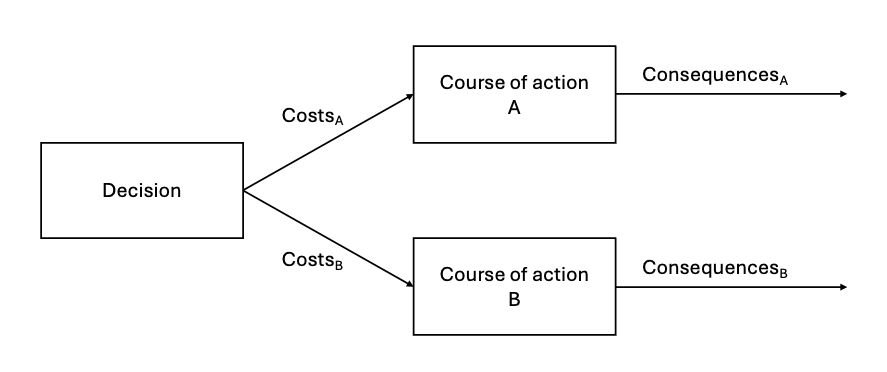
\includegraphics[width=1\linewidth]{core-chapters/figs/ch-1-fig-1.png}
    \caption{Illustration of the structure of health economic evaluations.}
    \label{fig:ch-1-fig-1}
\end{figure}

Study types for health economic evaluations vary based on the type of question they aim to inform, and the way health outcomes are measured. Several types are used in decision-making. These include \textit{cost-utility analysis} (CUA), \textit{cost-effectiveness analysis} (CEA), and \textit{cost-benefit analysis} (CBA). These three methods differ based the how health outcomes are valued, which can be in utility-weighted survival units (for CUA), health units (for CEA), or monetary units (for CBA). Other common types of analysis include \textit{cost-minimisation analysis} (CMA), where consequences are assumed to be equivalent and only costs are considered, and \textit{cost analysis}, a partial evaluation methods that compares costs only.

Debate persists about whether health economic evaluation should be \textit{welfarist} or \textit{extra-welfarist} in its approach.\cite{brouwer_welfarism_2008} Welfarist evaluations are concerned with maximising welfare and value all consequences with equivalent wellbeing equally. These evaluations consider all aspects of society and often take a \textit{societal perspective} in their analysis, including costs and consequences directly related to the individual, the health system, and non-health sectors. Extra-welfarist evaluations are concerned with maximising health outcomes and are typically undertaken from the \textit{health system perspective}, including only the consequences related to an individual’s health and the costs to the health system.

Regardless of the economic method, theoretical framework, or perspective chosen, health economic evaluations evaluate interventions in terms of their value-for-money and answer questions about the costs and consequences of competing alternatives. Historically, they have not included environmental impacts.

\subsection{Health technology assessment}
\textit{Health technology assessment} (HTA) is a process related to health economic evaluation that evaluates technologies in a specific decision context. It is used in many high-income countries with universal healthcare systems to inform decisions about government reimbursement. The International Network of Agencies for Health Technology Assessment (INAHTA) and Health Technology Assessment International (HTAi) define HTA as:
\begin{quote}
    ``a multidisciplinary process that uses explicit methods to determine the value of a health technology at different points in its life cycle. The purpose is to inform decision-making in order to promote an equitable, efficient, and high-quality health system."\cite{orourke_new_2020}
\end{quote}

HTA is used to inform decisions about which technologies are made available under one of the Australia’s universal access schemes: the Pharmaceutical Benefits Scheme (PBS), Medicare Benefits Schedule (MBS), National Immunisation Program (NIM), National Blood Agreement, or Prescribed List (PL), previously known as the prostheses list. HTA for this purpose is undertaken by the Pharmaceutical Benefits Advisory Committee (PBAC),\cite{australian_government_department_of_health_disability_and_ageing_guidelines_2016} Medical Services Advisory Committee (MSAC),\cite{australian_government_department_of_health_disability_and_ageing_guidelines_2021} and the Medical Devices and Human Tissue Advisory Committee (MDHTAC), who evaluate proposals submitted to them from applicants, such as pharmaceutical companies or device manufacturers. These committees advise the Minister for Health on whether, and under what circumstances, a technology should be recommended for reimbursement.\cite{australian_government_department_of_health_disability_and_ageing_guidelines_2016, australian_government_department_of_health_disability_and_ageing_guidelines_2021} The advice is primarily based on the comparative safety, effectiveness, cost-effectiveness (i.e., opportunity cost), and total cost of the technology, a focus that is common in HTA conducted for government reimbursement globally.\cite{world_health_organization_2015_2015}

Information about cost-effectiveness is obtained from within-trial and modelled economic evaluations of the health technology and its comparator. As with economic evaluation, environmental impacts have not traditionally been considered in HTA. However, there is interest in Australia and globally in understanding if this can be done.\cite{australian_government_department_of_health_and_aged_care_health_2024}

\section{Healthcare and climate change}
Health and climate change are connected in two ways. First, climate change has severe impacts on human health, and these are expected to worsen as the impacts of climate change continue. Second, health systems have large environmental impacts and are significant contributors to the greenhouse gas emissions causing climate change.

\subsection{Health impacts of climate change}
\textit{Climate change} is the ongoing increase in the Earth’s average temperature and its related impacts on weather and climate. The current period of climate change is being caused by human activity, primarily from \textit{greenhouse gas} (GHG) \textit{emissions}, such as carbon dioxide ($CO_{2}$), since the Industrial Revolution. The Sixth Report of the Intergovernmental Panel on Climate Change, released in 2023, found that global GHG emissions were the highest on record and that in the last decade average temperatures were 1.1 °C above pre-industrial levels.\cite{lee_climate_2023}

This increase in temperature is having devastating impacts on human health. The 2024 report of the Lancet-Countdown on health and climate change found record-breaking impacts to health and wellbeing.\cite{romanello_2024_2024} This includes direct impacts from heat, extreme weather events, infectious diseases, and food insecurity, and broader indirect economic and societal impacts.\cite{romanello_2024_2024}

Preventing the worst health impacts of climate change requires rapid reductions in GHG emissions to prevent further temperature increases. This is the ambition of the Paris Agreement, in which parties to the United National Framework Convention on Climate Change agreed to limit warming to 1.5 °C or well below 2 °C by achieving net-zero GHG emissions by 2050.

\subsection{Healthcare sustainability}
\textit{Healthcare sustainability} is variably defined and is generally used to describe efforts to reduce the environmental and climate change impact of the health system. It is focused on the demand and supply of healthcare technologies, mitigation and adaptation strategies, and decisions made at individual and system levels.\cite{mortimer_sustainable_2010, macneill_planetary_2021} This thesis is only concerned with matters of \textit{environmental sustainability} and how these relate to health technology assessment and health economic evaluation. We do not consider other types of sustainability that might also be covered by the label of ``healthcare sustainability".

The health sector has large environmental impacts. It accounts for about 5\% of national GHG emissions and in most countries is only exceeded by sectors related to energy, construction, and transport.\cite{pichler_international_2019, lenzen_environmental_2020} This is especially true for high-income countries with large health systems. In Australia, healthcare is responsible for 5\% to 7\% of total emissions.\cite{malik_carbon_2018, de_sain_estimates_2024} Most of this comes from the indirect impact of purchased goods and services required to deliver care, with only 27\% being attributable to direct emissions or energy use.\cite{de_sain_estimates_2024}

In a paper outlining the Campaign for Greener Healthcare in the United Kingdom, Mortimer identified four principles of sustainable clinical practice, as (1) disease prevention and health promotion, (2) patient education and empowerment, (3) lean service delivery, and (4) preferential use of treatment options and medical technologies with lower environmental impacts.\cite{mortimer_sustainable_2010} A recent framework by MacNeil, McGain \& Sherman describes a sustainable health system as one that reduces the demand of health services, matches supply of health services to demand, and reduces emissions from supply of health services.\cite{macneill_planetary_2021} Both of these approaches to sustainable healthcare emphasise decisions about the type of health technologies provided—decisions that can be informed by HTA. 

\section{Healthcare sustainability and health technology assessment}
Mortimer was one of the first to suggest healthcare decisions ought to consider environmental impacts, arguing in 2010 that the “inclusion of sustainability measures in the evaluation of medical technologies will allow service planners, clinicians and patients to choose clinically effective treatments with the best environmental profile and will encourage their further development.”\cite{mortimer_sustainable_2010} Mortimer did not suggest how this could be done, and it was several years before these ideas were developed further.

Between 2016 and 2020, health economists made substantial contributions to the question of whether environmental impacts can be used to inform health technology assessment, justifying several approaches and proposing methods for how it could be achieved. Marsh et al. were the first to argue that including environmental impacts in HTA is feasible from an economic perspective, outlining several methods that could be used to do so.\cite{marsh_expanding_2016} In a separate study, Marsh et al. demonstrated a simple method to include GHG emissions impacts in a modelled CEA, reporting total and incremental GHG emissions.\cite{marsh_incorporating_2016} This was the first empirical study demonstrating a method to include GHG emissions in a health economic evaluation. Later, de Preux and Rizmie demonstrated a similar method into include GHG emissions, but went a step further, valuing them in monetary units and including them as a cost in the incremental cost effectiveness ratio.\cite{de_preux_beyond_2018} In 2020, Hensher expanded on the work by Marsh et al. by also demonstrating the feasibility of valuing GHG emissions in monetary units.\cite{hensher_incorporating_2020}

In recent years there has been a considerable increase in the number of studies addressing the inclusion of environmental impacts in HTA and economic evaluation,\cite{polisena_environmental_2018, pinho-gomes_incorporating_2022, guirado-fuentes_main_2023, desterbecq_inclusion_2023, antonazzo_health_2025} and a detailed review of this literature is provided in Chapter \ref{ch-4} of this thesis. Much of this work is not specific to the Australian healthcare reimbursement decision-making context. 

\subsection{Australian policy context}
In Australia, HTA conducted to inform public reimbursement decisions are submitted by applicants for evaluation to the Medical Services Advisory Committee (MSAC) for medical interventions, the Pharmaceutical Benefits Advisory Committee (PBAC) for pharmaceuticals, and the Medical Devices and Human Tissue Advisory Committee (MDHTAC) for medical devices.

While these HTA focus on clinical and economic concerns, MSAC are currently able to consider other factors, including any relevant \textit{environmental aspects} of the technology.\cite{australian_government_department_of_health_disability_and_ageing_guidelines_2021} Guidelines for submissions to MSAC state, “if there are particular concerns regarding the environmental impact of the proposed health technology, or a key benefit in the way the proposed technology reduces the environmental impact compared with the comparator, these can be outlined”.\cite{australian_government_department_of_health_disability_and_ageing_guidelines_2021} It is therefore possible for MSAC to consider environmental impacts, however there is no evidence that this is being done, and MSAC has no further guidance on the topic. Guidelines for HTAs reviewed by PBAC and MDHTAC are silent on this matter and do not consider environmental aspects in their deliberations.\cite{australian_government_department_of_health_disability_and_ageing_guidelines_2016}

The Health and Climate Strategy, published in 2023, commits the Australian Government to review options to report and consider environmental impacts of health technologies in collaboration and alignment with international counterparts,\cite{australian_government_department_of_health_disability_and_ageing_national_2023} and this commitment was prioritised for implementation in 2024.\cite{australian_government_department_of_health_disability_and_ageing_national_2024} The Health Technology Assessment Policy and Methods Review, published in 2024, recommends the Australian Government investigate reporting environmental impacts during the assessment of cost-effectiveness and the potential to use this information in approval and reimbursement decisions.\cite{australian_government_department_of_health_and_aged_care_health_2024}

Despite these policies, there has been very little work to understand methods to include environmental impacts in HTA for the Australian context. 

\section{Case studies}
Two case studies for assessing environmental impacts were relied on throughout this thesis, both of which relate to the management of patients treated for melanoma of the skin. Australia has the highest incidence of melanoma in the world and this is a significant and growing health burden. After treatment, patients have a high risk of developing new primary melanomas and/or recurrence from their initial melanoma. Recommendations for the management of patients after treatment vary but include routine monitoring of the skin (to detect in-transit metastases or lymph node recurrence and new primary melanomas) and routine diagnostic imaging (to detect nodal or distant recurrence). 

The first case study involves the routine follow up of patients previously diagnosed with American Joint Committee on Cancer (AJCC) stage 0-II melanoma. The MELanoma SELF surveillance (MEL-SELF) randomised controlled trial (RCT) aimed to determine whether patient-led surveillance (smartphone supported skin self-examination, fast-tracked unscheduled visits as needed, usual care) compared with clinician-led surveillance (usual care), increases the proportion of participants diagnosed with a subsequent new primary melanoma at a fast-tracked unscheduled clinic visit.\cite{ackermann_can_2021} A pilot MEL-SELF RCT was previously completed.\cite{ackermann_assessing_2022} 

The second case study involves the routine follow up of patients previously diagnosed with AJCC stage III melanoma. After initial surgical treatment, patients undergo frequent diagnostic imaging tests, including positron emission tomography with computed tomography (PET/CT), to detect recurrent disease. A cohort of patients treated for stage III melanoma at the Melanoma Institute Australia between 2000 and 2014 was investigated.

\section{Objective}
The overall aim of this thesis is to evaluate methods to include environmental impacts in health economic evaluations and health technology assessments in the Australian reimbursement decision-making context.

The primary aims of the substantive parts of this thesis are to:
\begin{itemize}
    \item Describe potential methods to include environmental impacts in health economic evaluations and health technology assessments
    \item Demonstrate and evaluate methods to include environmental impacts in health economic evaluations
    \item Evaluate methods to include environmental impacts in Australian health technology assessment
\end{itemize}

\printbibliography[heading=subbibliography]
\end{refsection}